\begin{blocksection}
For the circuit below, assume: \\
    1. setup time is 15ns \\
    2. hold time is 30ns \\
    3. AND gate delay is 10ns.  \\
If the clock rate is 10 MHz and x updates 25ns after the rising edge of the clock,what are the minimum and maximum values for the clk-to-Q delay to ensure proper functionality?
    
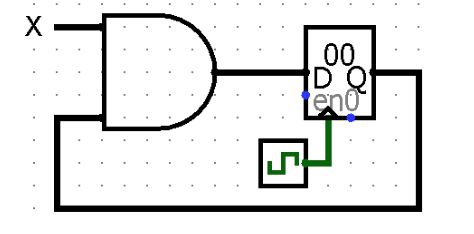
\includegraphics[width=\textwidth]{images/sds/holdtime.png}

\item Min: $\rule{1.5cm}{0.15mm}$ ns
\item Max: $\rule{1.5cm}{0.15mm}$ ns

\begin{solution} 
Min: 20 ns \\
Max: 75 ns

If the clk-to-Q delay is too fast, the input to the register will change before the hold time is finished.
Thus, the minimum clk-to-Q delay is $t_{hold} – t_{and} = 30 – 10 = 20$ ns.
On the other hand, we must make sure the critical path is no longer than the clock period, which is $100 ns (= 1/(10 MHz))$. 
In other words, $t_{setup} + t_{and} + t_{clk-to-Q} \leq 100ns$, or $tclk-to-Q \leq 100ns - t_{setup} - t_{and}$. Solving yields $t_{clk-to-Q} \leq 75 ns$.
    
\end{solution}
    
\end{blocksection}